
\chapter{Background}

The paradigm "Earth System Science" (or simply "Earth System") acknowledges that changes in the solid earth 
(land - lithosphere or geosphere) result from interactions among the atmosphere (air), hydrosphere (water, including oceans, rivers, ice), 
biosphere (life) and the lithosphere~\cite{introgeo}.
%(Two additional elements are the human dimension (or anthroposphere) and 
%the solar system and interplanetary space (or exosphere)). 


\begin{figure}[h!]
    \centering
    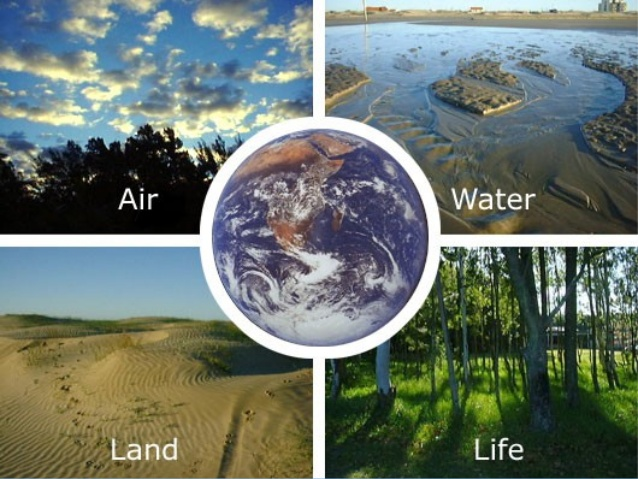
\includegraphics[scale=0.35]{pic/intro}
    \caption{The Earth system}
    \label{fig:ecearth}
\end{figure}



Earth System Science also includes studies of the ways energy and materials cycle through the different "-spheres" 
as well as the workings of climate and the biosphere. Solid earth geoscientists will be familiar with "The Rock Cycle" 
which appears in almost every introductory geology book. Earth system science, by contrast, shows how elements like 
carbon or energy sources like solar radiation cycle through the lithosphere and all of the other "-spheres."  (see Figure~\ref{fig:schema})
\begin{figure}[!hp]
    \begin{minipage}[c]{0.54\linewidth}
        \centering
        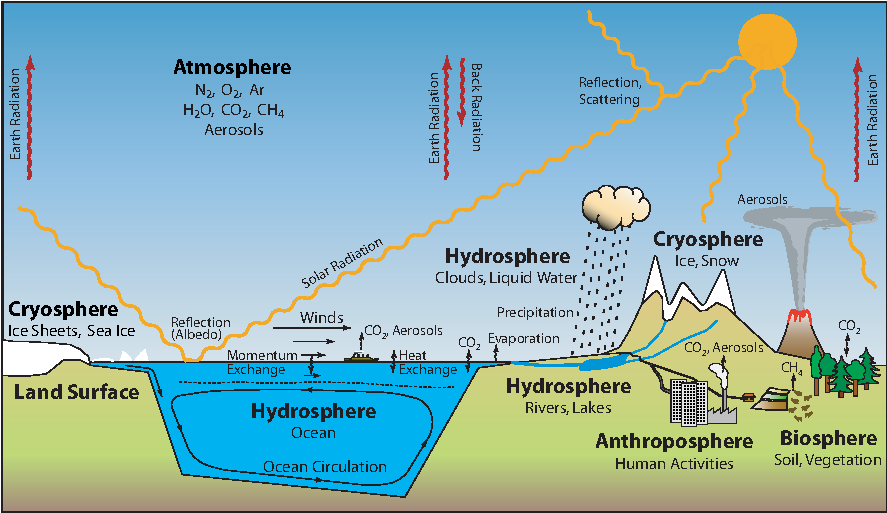
\includegraphics[scale=0.6]{pic/cycle}
    \end{minipage}
    \begin{minipage}[c]{0.45\linewidth}
        \centering
        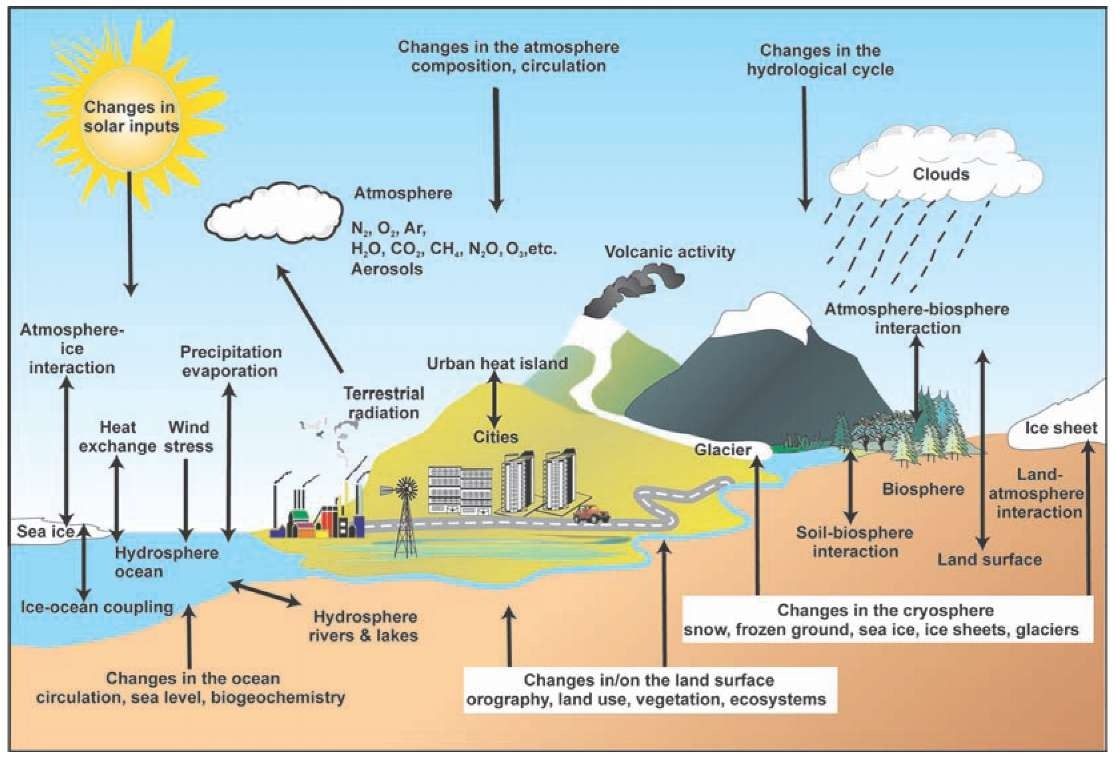
\includegraphics[scale=0.6]{pic/tmp6441}
    \end{minipage}  
    \caption{Schematic view of the components of the climate system, their processes and interactions~\cite{Stocker2011,ipcc}.}
    \label{fig:schema}
\end{figure}


Climate models are a mathematical representation of the climate. In order to be able to do this, the models divide 
the earth, ocean and atmosphere into a grid. The values of the predicted variables, such as surface pressure, wind, 
temperature, humidity and rainfall are calculated at each grid point over time, to predict their future values. 
The time step (the interval between one set of solutions and the next) is a function of the grid size: the finer the 
resolution the shorter the interval between each computation. For example, a model with a 100 km horizontal resolution 
and 20 vertical levels, would typically use a time-step of 10--20 minutes. A one-year simulation with this configuration 
would need to process the data for each of the 2.5 million grid points more than 27 000 times -- hence the necessity 
for supercomputers. In fact it can take several months just to complete a 50 year projection. 

When it comes to simulating the general behaviour of the climate system over lengthy periods, however, 
it is essential to use models that represent, and where necessary conserve, the important properties of the 
atmosphere, land surface and the oceans in three dimensions. At the interfaces, the atmosphere is coupled to the land 
and oceans through exchanges of heat, moisture and momentum. These models of the climate system are usually known as coupled global climate models (GCMs)~\cite{wmo-models}.

\begin{figure}[!hp]
    \centering
    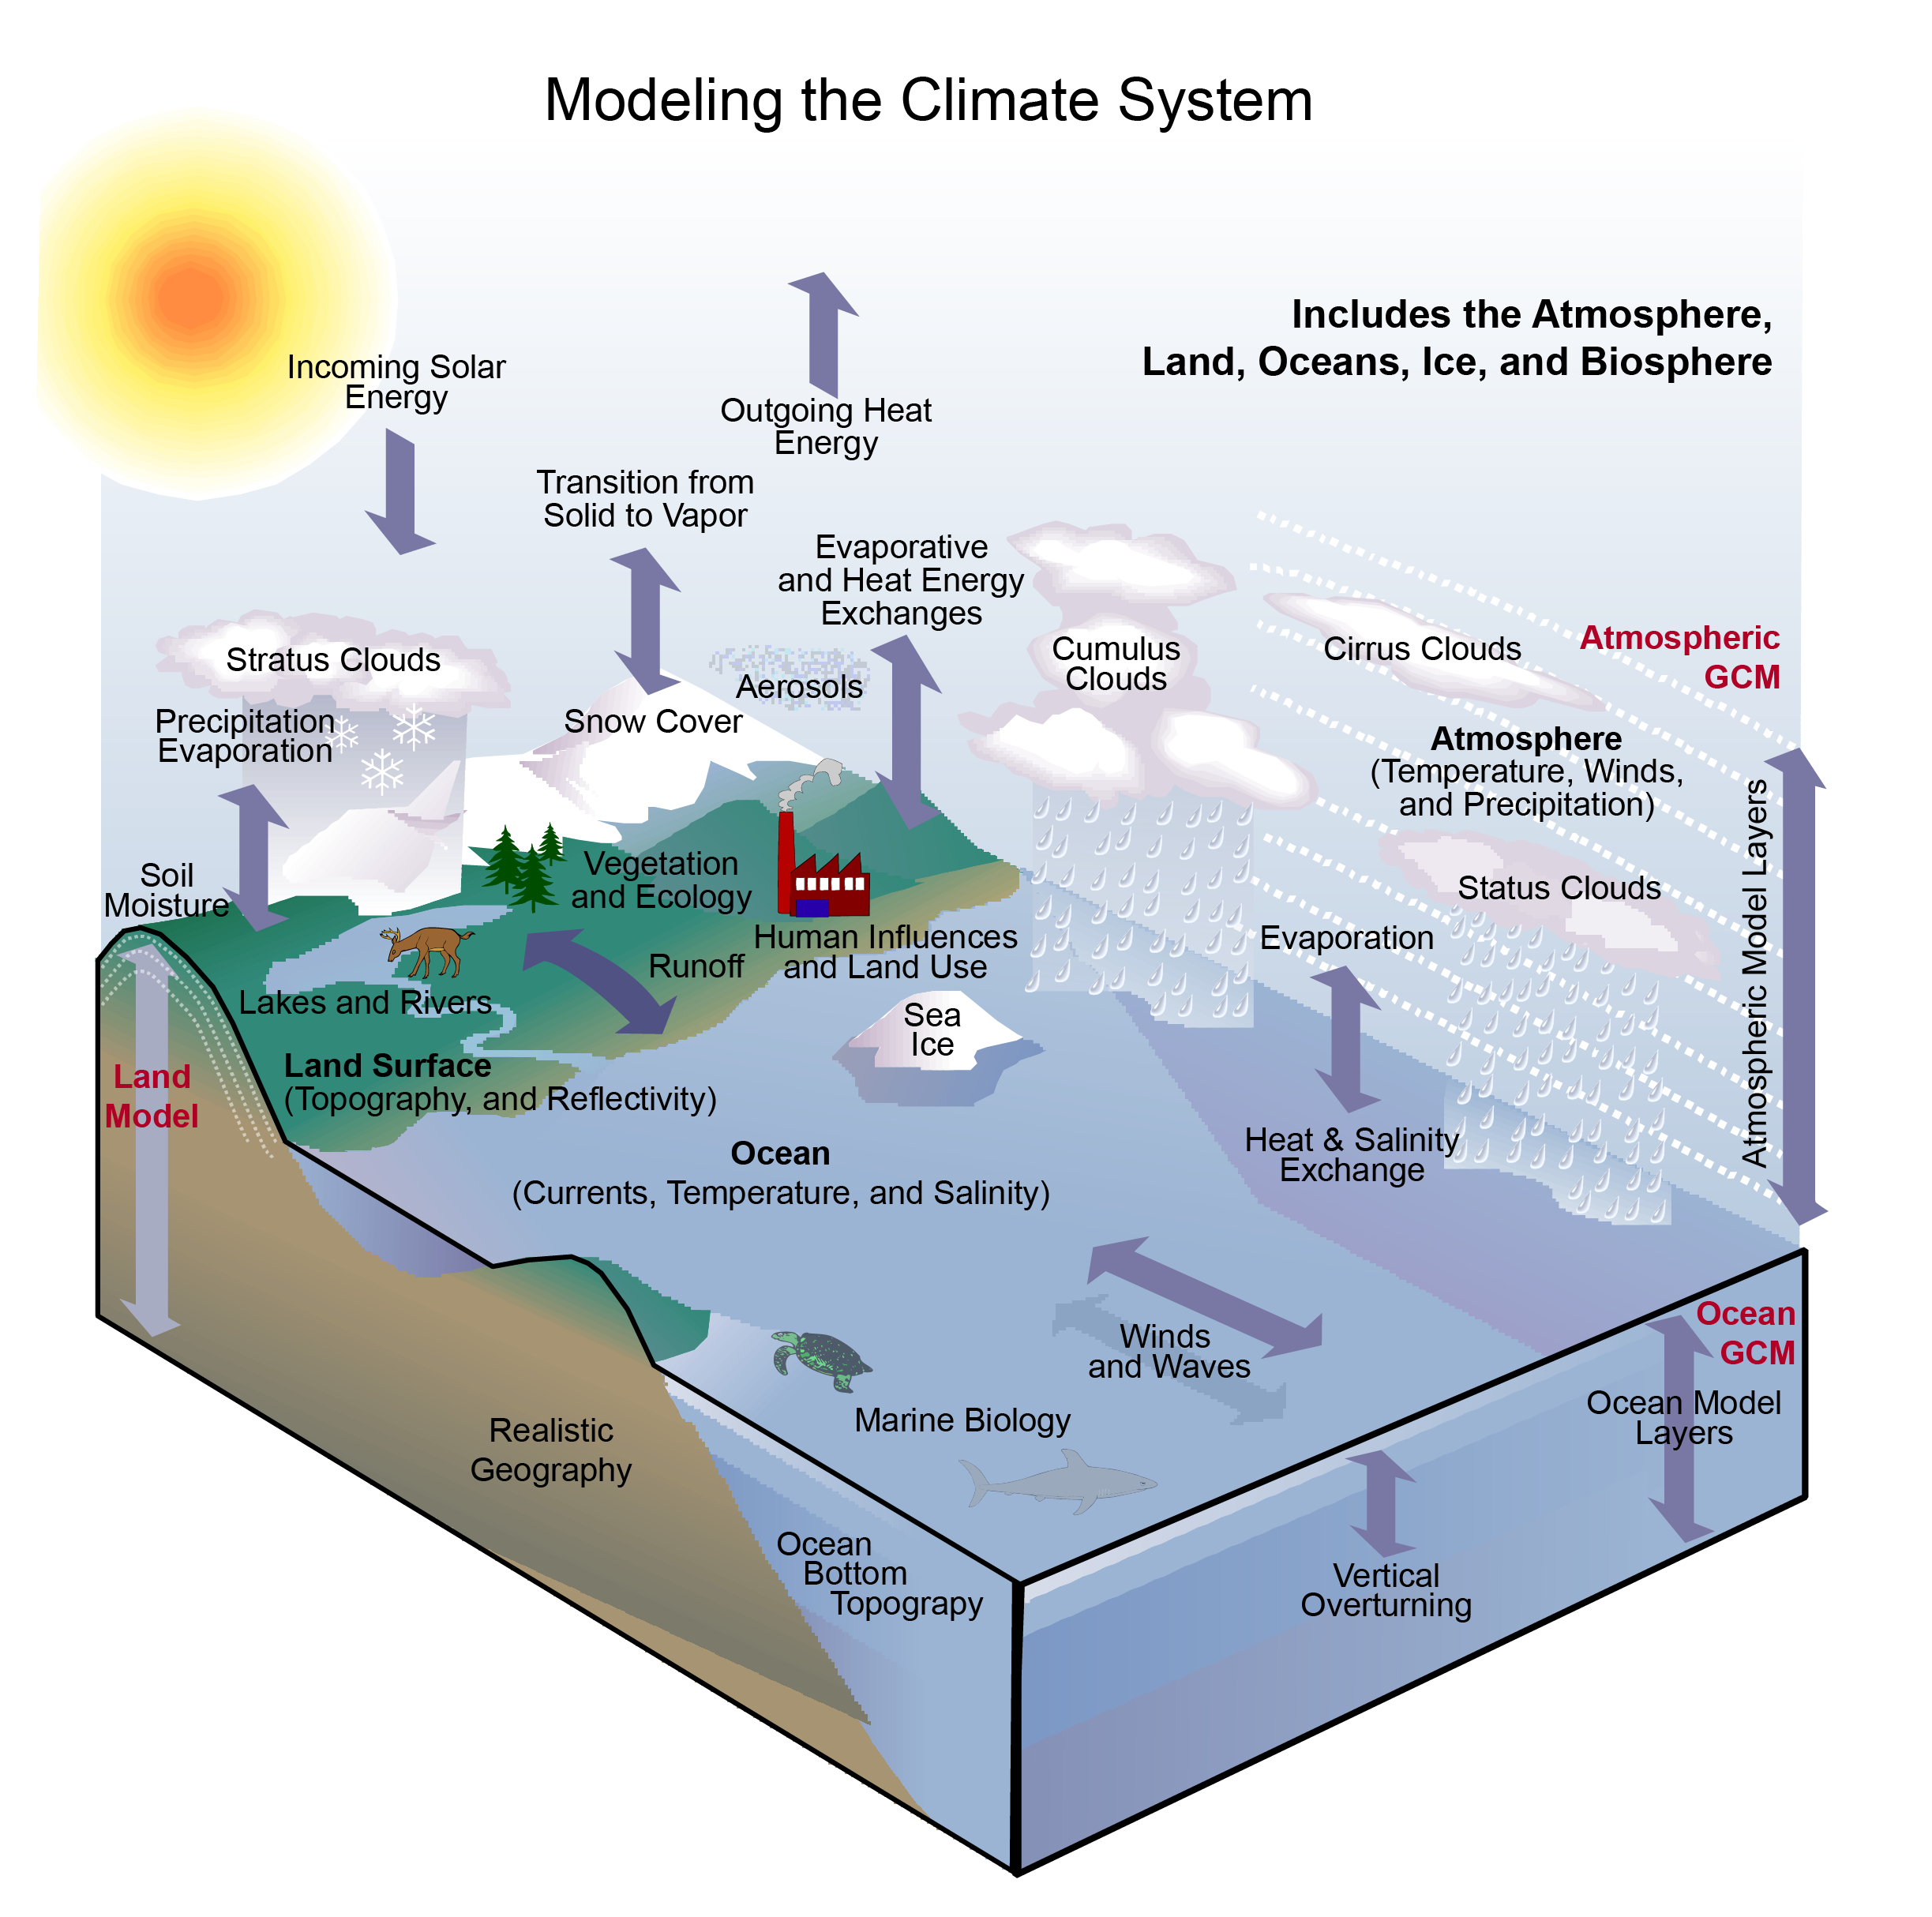
\includegraphics[scale=0.6]{pic/APP_modeling_the_climate_V2}
    \caption{Modeling the Climate System: Some of the many processes often included in models of the Earth's climate system \cite{KT2003})}
    \label{fig:schema2}
\end{figure}

Coupling the ocean processes to atmospheric GCMs is a major challenge. The thermal capacity of the oceans is massive compared to 
the atmosphere and can provide to, or extract from, the atmosphere, massive amounts of latent and thermal heat. Representing their 
heat storage, and the absorption of greenhouse gases by the oceans, in long-term simulations of climate requires a full three-dimensional 
ocean model, which simulates even the deep currents. Changes in the intensity and location of deep-water currents can ultimately have 
profound effects on the atmosphere. In the past, changes in the circulation of the oceans have produced major atmospheric responses. 





\section{Architecture}
%Components and their descriptions
EC-Earth~\cite{Hazeleger2010,Hazeleger2012} is an Earth system model implemented in a scientific software development project. %
% src: https://verc.enes.org/models/earthsystem-models/ec-earth-1/ec-earth
It is developed by the EC-Earth consortium, gathering a number of national weather services 
and universities from currently 11 countries in Europe. EC-Earth component models are IFS for the atmosphere, 
NEMO for the ocean, and LIM for the sea-ice, coupled through OASIS, and so on (see Figure~\ref{fig:ecearth}). 



\begin{figure}[h!]
    \centering
    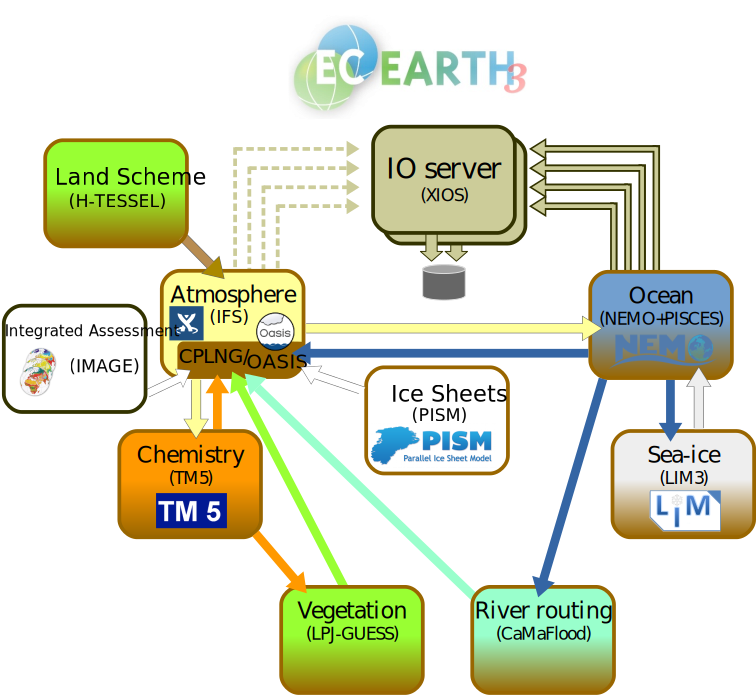
\includegraphics[scale=0.5]{figs/cw2015-ec-earth}
    \caption{Earth cycle}
    \label{fig:ecearth}
\end{figure}

EC-Earth is used in coordinated model intercomparison projects (e.g. CMIP6) to make projections and predictions 
of near-term and end-of-the-century climate change and variability. The data is downscaled to a local level for 
Climate Services by partners in different European countries (notably the Netherlands, Sweden, Denmark, Italy, Spain, 
Ireland). Also many sensitivity studies are conducted.


EC-Earth (version 3.2) consists of multiple components, some of which can be run standalone:
\begin{itemize}
    \item IFS: representing the atmosphere;
    \item NEMO (3.6) representing the ocean;
    \item LIM (3): representing the sea-ice, is a part of ocean model;
    \item HTESSEL: representing the continental surfaces and vegetation;
    \item TM5: representing the atmospheric chemistry;
    \item the coupler OASIS3-MCT;
    \item scheme for runoff coupling between atmosphere and ocean.
\end{itemize}

\subsection{IFS}
The IFS uses a linear reduced Gaussian grid for computation in grid point space. All prognostic variables are co-located at the grid points of the Gaussian grid~\cite{ifs-meta}.

GRIB data is archived in one of the following spatial coordinate systems~\cite{spatial-ecmwf}:   
\begin{itemize}
    \item Spherical Harmonics (SH) - Upper air fields.
    \item Gaussian Grid (GG) - Surface and some upper air fields.
    \item Latitude/Longitude (LL) - other centres, wave data.
\end{itemize}
The correspondence between the three types of grid resolutions is as shown in Table~\ref{tab:spac-coord}.
    
\begin{table}[h!]
\centering
\begin{tabular}{|l|c|c|}
    \hline      
    Spectral  & Gaussian  & Lat/lon\\
    \hline
    T63  & N48  & 1.875\\
    TL95  & N48  & 1.875\\
    T106  & N80  & 1.125\\
    TL159  & N80  & 1.125\\
    T213  & N160  & 0.5625\\
    TL255  & N128  & 0.7\\
    TL319  & N160  & 0.5625\\
    TL399  & N200  & 0.450\\
    TL511  & N256  & 0.351\\
    TL639  & N320  & 0.28125\\
    TL799  & N400  & 0.225\\
    TL1023  & N512  & 0.176\\
    TL1279  & N640  & 0.141\\
    TL2047  & N1024  & 0.088\\  
    \hline
\end{tabular}
\caption{Data spatial coordinate systems}
\label{tab:spac-coord}
\end{table}  

\begin{table}[h!]
\centering       
\begin{tabular}{|l|c|c|c|c|c|c|c|c|}
    \hline 
    Model resolution & 159 & 255 & 319 & 399 & 511 & 639 & 799 & 1279 \\
    \hline
    Radiation grid & 63 & 95 & 159 & 159 & 159 & 255 & 319 & 511 \\
    Time-step & 3600 & 2700 & 1800 & 1350 & 1200 & 900 & 720 & 600 \\
    \hline
\end{tabular} 
\caption{Radiation grid and time-step for the IFS at different horizontal resolutions} 
\label{tab:ifs-grid}
\end{table}
Table~\ref{tab:ifs-grid} presents the model horizontal resolution, radiation grid resolution and time-step in the various configurations of the IFS from T159 to T1279~\cite{1399454274743}.


Also, IFS has stochastic physics flag. 

TODO:  IFS model levels

\subsection{NEMO}

NEMO (Nucleus for European Modelling of the Ocean)~\cite{nemo-book36}

In the form suitable for running on massively-parallel architectures, NEMO is a Fortran90 code that uses the Message Passing Interface (MPI) library for inter-process
communication. When running a whole-Earth configuration, the PEs along the northern-most boundary of the domain are collected into an additional MPI communicator. Further
computation and communication is performed within this communicator to deal with the boundary conditions imposed by the poles~\cite{nemo-report}. In NEMO, the mesh poles are moved to land points~\cite{ref1}.

LIM3~\cite{lim36,gmd-8-2991-2015}



\begin{table}[h!]
\centering
\begin{tabular}{|l|c|c|c|}
    \hline 
    name    & npi  & npj  & points  \\
    \hline   
    ORCA2   & 182  & 149  & 27118   \\
    ORCA1   & 362  & 292  & 105704  \\
    ORCA05  & 722  & 511  & 368942  \\
    ORCA025 & 1440 & 1021 & 1470240 \\
    \hline
\end{tabular}
\caption{Number of rows, columns and total number of horizontal grid points for the different resolutions of the ORCA grid~\cite{oriol14}.}
\label{tab:nemo-grid}
\end{table}

TODO:Nemo grid size further

\subsection{OASIS}
%\cite{Alexander2011}
Since the climate system is highly interconnected, EC-Earth requires code to tie the components together - interpolating fluxes between grids and controlling interactions between components. These tasks are performed by the coupler.

OASIS is a software interface to couple existing ocean and atmosphere models. At run-time, OASIS3-MCT~\cite{oasis3-mct} allows exchanging coupling data between two components as well as interpolation and transformation of these coupling fields. 

TODO: Oasis frequency


\subsection{CMIPs}
% src: http://cmip-pcmdi.llnl.gov/
Under the World Climate Research Programme (WCRP) the Working Group on Coupled Modelling (WGCM) established the Coupled Model Intercomparison Project (CMIP) as a standard experimental protocol for studying the output of coupled atmosphere-ocean general circulation models (AOGCMs). CMIP provides a community-based infrastructure in support of climate model diagnosis, validation, intercomparison, documentation and data access. This framework enables a diverse community of scientists to analyze GCMs in a systematic fashion, a process which serves to facilitate model improvement. Virtually the entire international climate modeling community has participated in this project since its inception in 1995. T
Coupled atmosphere-ocean general circulation models allow the simulated climate to adjust to changes in climate forcing, such as increasing atmospheric carbon dioxide. CMIP began in 1995 by collecting output from model "control runs" in which climate forcing is held constant. Later versions of CMIP have collected output from an idealized scenario of global warming, with atmospheric CO2 increasing at the rate of 1\% per year until it doubles at about Year 70. CMIP output is available for study by approved diagnostic sub-projects. 
CMIP has developed in phases, with the simulations of the fifth phase, CMIP5, now mostly completed. Current phase of the project is 6, i.e. CMIP6. 

For more information on CMIP5 models and their resolutions, we refer to~\cite{cmip5}.

\section{Input data}
%   Resolution description, its list and the description of each file, grid type

\subsection{Resolutions and grid sizes}
See Tables~\ref{tab:ifs-grid},~\ref{tab:nemo-grid},~\ref{tab:spac-coord}.

The \texttt{namcouple.sh} file contains the following information regarding IFS and NEMO:

\begin{lstlisting}
    159) atm_grid=A080
        atm_nx=35718
        ;;
    255) atm_grid=A128
        atm_nx=88838
        nem_nx=362
        nem_ny=292
        ;;
    511) atm_grid=A256
        atm_nx=348528
        nem_nx=1442
        nem_ny=1021
        ;;
    799) atm_grid=A400
        atm_nx=843490  
\end{lstlisting}




% TODO: Refernence to nemo internal doc from namcouple




\section{Internal algorithms}
Solver algorithms choices